%*****************************************************************************************
% STUFFS
%*****************************************************************************************
\documentclass{article}
\usepackage{times}
\usepackage{latexsym}
\usepackage{amsfonts}
\usepackage{amsmath} 
\usepackage{pifont}
\usepackage{subfig}
\usepackage[utf8]{inputenc} 													
\usepackage[T1]{fontenc}     			 															
\usepackage{graphicx}		
\usepackage{amssymb}		
\usepackage{textcomp}																						
\usepackage{amsmath}		
\usepackage{algorithm}
\usepackage{cancel}
\usepackage{algpseudocode}
\usepackage{multirow}
\usepackage{latexsym}
\usepackage{xcolor}
\usepackage{listings}
\usepackage{authblk}
\usepackage{hyperref}
\hypersetup{
    colorlinks,
    citecolor=black,
    filecolor=black,
    linkcolor=black,
    urlcolor=black
}

% Tikz
\usepackage{pgfplots}
\usepackage{tikz}
\usetikzlibrary{calc}
\tikzstyle{myLabel}=[minimum height=\myShiftHeight, anchor=south west]
\tikzstyle{myLDashed}=[draw, loosely dashed]
\tikzstyle{myDDashed}=[draw, densely dashed]
\tikzstyle{myAxis}=[draw, ->]
\tikzstyle{vertex}=[circle,draw,fill=black!25,minimum size=10pt,inner sep=0pt]
\tikzstyle{selectedVertex}=[circle,fill=white,draw,thick,minimum size=15pt,inner sep=0pt]
\tikzstyle{edge} = [draw,-]
\tikzstyle{weight} = [font=\small]

% --- 
\begin{document}
%*****************************************************************************************
% TITLE
%*****************************************************************************************
\author[1]{Jean-Guillaume Fages}
\author[2]{Charles Prud'homme}
\author[2]{Xavier Lorca}
\affil[1]{\small{\href{https://www.cosling.com/}{COSLING} S.A.S., https://www.cosling.com/}}
\affil[2]{\small{\href{http://web.emn.fr/x-info/ppc/index_en.html}{TASC} research team, IMT Atlantique, https://www.imt-atlantique.fr/}}                      
\title{Choco Graph Documentation \\ \large{Choco Solver module for graph variables (version 4.2.2)}}
\maketitle

\begin{abstract}
This document describes the API  of Choco-Graph, a module of the Choco Solver \cite{choco} which enables to search for a graph subject to constraints. 
It explains how to create graph variables and uses available graph constraints and search procedures. It also describes how to build your own ones. Finally, a few examples are provided.

This solver is an output of the PhD Thesis of \cite{FagesPhD,FagesPhDFr}. Other references to graph variables may be found in the litterature \cite{Beldiceanu00,LorcaBook11,ReginSlides04,QuesadaPhD,DoomsPhD} but they are based on a different implementation. 

\emph{This document assumes the reader is already familiar with the concepts of Constraint-Programming \cite{CPhandbook} and the Choco Solver.}
\end{abstract}

\newpage{}
{\scriptsize\tableofcontents{}}
\newpage{}

\newcommand{\GV}{\ensuremath{\mathcal{G}}}
\newcommand{\GLB}{\ensuremath{\underline{\mathcal{G}}}}
\newcommand{\GUB}{\ensuremath{\overline{\mathcal{G}}}}

\definecolor{javared}{rgb}{0.6,0,0} % for strings
\definecolor{javagreen}{rgb}{0.25,0.5,0.35} % comments
\definecolor{javapurple}{rgb}{0.5,0,0.35} % keywords
\definecolor{javadocblue}{rgb}{0.25,0.35,0.75} % javadoc

\section{Introduction}

\subsection{Overview}

This \href{http://www.choco-solver.org/}{Choco Solver} module allows you to search for a graph\footnote{Either directed or undirected, with at most one arc/edge between any two vertices. }, which may be subject to constraints. 
%
The domain of a graph variable \GV{} is a graph interval $[\GLB{},\GUB{}]$. \GLB{} is the graph representing vertices and edges which must belong to any single solution whereas \GUB{} is the graph representing vertices and edges which may belong to one solution. Therefore, any value $\GV{}^*$ must satisfy the graph inclusion $\GLB{} \subseteq \GV{}^* \subseteq \GUB{}$. One may see a strong connection with set variables.
%
A graph variable can be subject to graph constraints to ensure global graph properties (e.g. connectedness, acyclicity) and channeling constraints to link the graph variable with some other binary, integer or set variables. 
%
The solving process consists of removing nodes and edges from \GUB{} and adding some others to \GLB{} until having $\GLB{} = \GUB{}$, i.e. until \GV{} gets instantiated. These operations stem from both constraint propagation and search. You may wonder why using a graph variable. Here are the most important motivations to do so:
\begin{itemize}
\item Modeling convenience : 
\begin{itemize}
\item When solving a graph problem, the model is close to the original problem. 
\item A graph variable is a consistent graph representation (e.g. a node which does not exist has no incident arcs), which simplifies the model. 
\item Stating constraints as graph properties in a declarative way is nice. 
\end{itemize}
\item Implementation convenience : 
\begin{itemize}
\item Manipulating a domain which consists of two graphs (representing respectively mandatory and potential elements) makes easy the implementation of graph-based filtering algorithms. As the implementation becomes more natural, the risk of mistakes decreases.
\end{itemize}
\item Performance gains : 
\begin{itemize}
\item You can use optimized data structure for domains (e.g. bit sets, bipartite sets, linked lists...) which allow to reduce runtime of most algorithms and/or memory consumption. This brings significant improvement on large scale problems. 
\item Having such a global variable instead of many smaller ones makes the solver lighter, which brings performance improvement.
\end{itemize}
\end{itemize}

This module can be seen as a CP framework for graph theory. In that sense, it is closer to Operations Research than Artificial Intelligence. With a minimum background in graph algorithms, this manual will help you to build your own models, constraints and search procedures so that you effectively solve your problems. 

%This module has been introduced in 2011 but it has been deeply refactored in September 2014. 


\subsection{How to cite Choco Graph?}

A reference to this manual, or more generally to Choco Graph, is made like this:
\lstset{language=Java,
basicstyle=\scriptsize{},
numbers=left,
frame=single,
numberstyle=\tiny\color{black},
stepnumber=0,
numbersep=10pt,
tabsize=4,
showspaces=false,
showstringspaces=false,
columns=fullflexible}
\begin{lstlisting}
@manual{chocograph,
  author        = {Jean-Guillaume Fages and Charles Prud'homme and Xavier Lorca},
  title         = {Choco Graph Documentation},
  year          = {2018},
  organization  = {COSLING S.A.S., IMT Atlantique},
  timestamp     = {Mon, 5 Mar 2018},
  url           = {https://github.com/chocoteam/choco-graph/},
}
\end{lstlisting}
\lstset{language=Java,
basicstyle=\scriptsize{},
keywordstyle=\color{javapurple}\bfseries,
stringstyle=\color{javared},
commentstyle=\color{javagreen},
morecomment=[s][\color{javadocblue}]{/**}{*/},
numbers=left,
frame=single,
numberstyle=\tiny\color{black},
stepnumber=0,
numbersep=10pt,
tabsize=4,
showspaces=false,
showstringspaces=false}

\subsection{Which version of Choco Solver?}

This extension should be used with Choco Solver 4.0.6

\subsection{Need support?}

The company \href{https://www.cosling.com/}{COSLING} can provide you with professional support and specific software development related to Choco Graph and Choco Solver. Feel free to contact our consultants at contact@cosling.com to discuss your upcoming projects.



If you encounter any bug, please feel free to open an issue on \href{https://github.com/chocoteam/choco-graph/}{GitHub}.

\newpage{}
\section{Defining a graph variable}

Prior to introduce how to build graph variables, it is necessary to describe graph structures of the core Choco solver. These graphs are often used as internal data structures for propagators. In our case, it will serve to define the domain of graph variables. 

\subsection{Graphs}

There are basically two kind of graphs in Choco : directed (\texttt{DirectedGraph.java}) and undirected (\texttt{UndirectedGraph.java}) graphs. 
Directed and undirected graphs have similar methods. The constructor of an undirected graph is the following: 
\begin{lstlisting}
public UndirectedGraph(int n, SetType type, boolean allNodes)
\end{lstlisting}

\begin{itemize}
\item The integer \texttt{n} denotes the maximum number of nodes. This is necessary for memory allocation. The set of nodes is then a subset of $\{0,1,...,n-1\}$. Once the graph has been created, it is not possible to modify that value. 
\item \texttt{SetType type} indicates which kind of data structure to use. If the graph is very sparse, a linked list (\texttt{SetType.LINKED\_LIST}) implementation would reduce the memory consumption. Otherwise, \texttt{SetType.BIPARTITESET} provides an optimal time complexity for every request, but has some hidden constants and a higher memory consumption. \texttt{SetType.BITSET} is a good default choice. 
\item The boolean \texttt{allNodes} indicates whether or not the node set is fixed. This parameter is very important. Whenever set to true, it means that the vertex set is $[0,n-1]$ and will not change during search. It is not necessary to add vertices explicitly (all of them are present). If set to false, it means that the vertex set must be a subset of $[0,n-1]$, and is initially EMPTY. Therefore, the user may have to add them explicitly by using the \texttt{addNode(int i)} method.
\end{itemize}

Graph manipulations (iterations over nodes, edges, neighbors of a particular vertex...) rely on the choco \texttt{ISet} interface. 
\begin{lstlisting}
for(int i:graph.getNodes()){
...
}
\end{lstlisting}
Note that for efficiency reason iteration of one \texttt{ISet} is not context safe, i.e. you cannot encapsulate two iteration loops of the same set because only one iterator is created by default (copy the set in an int[] for doing that, or create a new iterator explicitly).
\subsection{Backtrackable graphs}

As we wish to use graphs to represent the domain of a variable, such graphs must be backtrackable, i.e. the graph must restore its previous value upon backtracking. 
To do so, one simply use a different constructor, having the model in argument (to catch backtrack events):

Therefore, you should use the following signatures when creating domain bounds:
\begin{lstlisting}
new UndirectedGraph(Model model, int n, SetType type, boolean allNodes)
new DirectedGraph(Model model, int n, SetType type, boolean allNodes)
\end{lstlisting}

\subsection{Graph Model}

Since version 4, Choco Solver uses a \texttt{Model} object to create variables and constraints of the model, whereas the \texttt{Solver} object contains everything related to the solving process. In Choco Graph, the \texttt{Solver} object remains the same, but the model must be a \texttt{GraphModel} object, which inherits from \texttt{Model}:

\begin{lstlisting}
GraphModel model = new GraphModel();
\end{lstlisting}
\fbox{\color{blue}Almost everything will be accessible from \texttt{model.} + ctrl space (autocompletion)}

\subsection{Graph variable}

Graph variables can be created through the \texttt{GraphModel}. The domain of such a variable is defined by two graphs : the lower bound graph gives nodes and arcs that belong to every solution, whereas the upper bound graph gives nodes and arcs that may belong to a solution. \texttt{GraphModel} methods to create a graph variable:

\begin{lstlisting}

/**
 * Create an undirected graph variable named name
 * and whose domain is the graph interval [lb,ub]
 * BEWARE: lb and ub graphs must be backtrackable
 * (use the solver as an argument in their constructor)!
 *
 * @param name		name of the variable
 * @param lb		Undirected graph representing mandatory nodes and edges
 * @param ub		Undirected graph representing possible nodes and edges
 * @return	An undirected graph variable
 */
default UndirectedGraphVar graphVar(String name, 
								UndirectedGraph lb, 
								UndirectedGraph ub) {
	return new UndirectedGraphVar(name, _me(), lb, ub);
}

/**
 * Create a directed graph variable named name
 * and whose domain is the graph interval [lb,ub]
 * BEWARE: lb and ub graphs must be backtrackable
 * (use the solver as an argument in their constructor)!
 *
 * @param name		name of the variable
 * @param lb		Directed graph representing mandatory nodes and edges
 * @param ub		Directed graph representing possible nodes and edges
 * @return	An undirected graph variable
 */
default DirectedGraphVar digraphVar(String name, 
								DirectedGraph lb, 
								DirectedGraph ub) {
	return new DirectedGraphVar(name, _me(), lb, ub);
}
\end{lstlisting}

Note the the bound graphs must be backtrackable. The input maximum number of nodes should be the same for both the lower and the upper bound graphs. 
%
%The \texttt{Solver} provides a backtracking environment. You should NOT use the signatures that do not have the solver in argument (they do not restore value upon backtracking). The integer \texttt{n} denotes the maximum number of nodes. This is necessary for memory allocation. \texttt{SetType type} indicates which kind of data structure to use. Finally, the boolean \texttt{allNodes} indicates whether or not the node set is fixed. This parameter is very important. Whenever set to true, it means that the vertex set is $[0,n]$ and will not change during search. It is not necessary to add vertices explicitly. If set to false, it means that the vertex set must be a subset of $[0,n]$, and is initially EMPTY. Therefore, the user may have to add them explicitly (see the following example with \texttt{GUB.addNode(i);}).
%
Here is an example involving an undirected graph variable:

\begin{lstlisting}
// graph model 
GraphModel model = new GraphModel();
// graph variable domain
UndirectedGraph GLB = new UndirectedGraph(
										model,			// Restore value on backtrack
										n,				// Maximal number of nodes
										SetType.BITSET,	// data structure type
										false			// fixed node set?
									);
UndirectedGraph GUB = new UndirectedGraph(
										model,			// Restore value on backtrack
										n,				// Maximal number of nodes
										SetType.BITSET,	// data structure type
										false			// fixed node set?
									);
for (int i = 0; i < n; i++) {
	GUB.addNode(i);			// potential node
	for (int j = i; j < n; j++) {
		if (link[i][j]) {       // some input data providing potential edges
			GUB.addEdge(i, j);		// potential edge
		}
	}
}
GLB.addNode(1);				// 1 and 2 must belong to the solution
GLB.addNode(2);
GLB.addEdge(1,2);					// 1 and 2 must belong to the same clique
// graph variable
graphvar = model.graphVar("G", GLB, GUB);
\end{lstlisting}

In this example, we see that vertices $1$ and $2$ must belong to every solution, as well as the edge $(1,2)$. 
Other potential vertices and edges are given by \texttt{GUB}. 

For simplicity reasons, one may prefer to use the following method, which creates an empty lower bound graph and a complete upper bound graph with $42$ vertices:
\begin{lstlisting}
model.graphVar("G",42);
\end{lstlisting}

\newpage{}
\section{Constraining a graph variable}

A collection of constraints over a graph variable can be found in \texttt{GraphModel}, which implements \texttt{IGraphConstraintFactory}. 

\subsection{Usual graph constraints}

\subsubsection{Node and edge counts}

The factory contains several basic constraints, such as \texttt{nbNodes}, which enables to constrain the number of nodes to be equal to a given integer variable. 
To make things simpler, you can call the \texttt{model.nbNodes(g)} function which will create and return an integer variable that is equal to the number of nodes (i.e. it posts the \texttt{nbNodes} constraint). 
In the same way, one can count the number of edge (resp. arc) of an undirected (resp. directed) graph variable as follows: 
\begin{lstlisting}
// Creates an IntVar equal to the number of arcs in g
IntVar nbArcs = model.nbArcs(g);
or
// posts a constraint saying that the IntVar x is equal to the number of arcs in g
model.nbArcs(g,x).post(); 
\end{lstlisting}  

\subsubsection{Loops}

Graph variables may contain loops, i.e. arcs of the from $(i,i)$. If you want the graph to contain no loops, then you should simply make sure the graph upper bound has initially no loop. Instead, if you wish some vertices to have a loop, then you can use the \texttt{loopSet(g,l)} constraint which ensures that the set variable $l$ represents the nodes of $g$ that have a loop. You can also directly create that set variable using:
\begin{lstlisting}
SetVar loops = model.loopSet(graphvar);
\end{lstlisting} 

%every vertex to have a loop, then there are basically two options. If all vertices are mandatory, then you should simply make sure the graph lower bound has initially a loop on every node. Else, you can use the constraint \texttt{each\_no\_has\_loop(g)}. 
Finally, you can control the number of loops the graph variable has with an integer variable with the following : 
\begin{lstlisting}
IntVar nbLoops = model.nbLoops(g);
\end{lstlisting} 

\subsubsection{Degrees}

It is possible to constrain the minimum and the maximum degree each node of an undirected graph variable, by using respectively \texttt{minDegrees} and \texttt{maxDegrees} constraints. 
Such constraints only hold on vertices that belong to the solution. For instance, if vertex $a$ is constrained to have a degree greater than $5$ but has only $4$ potential neighbors, then vertex $a$ should be removed from the potential vertex set. Unless $a$ was a mandatory vertex, this does not trigger any failure. Here is an example imposing every vertex to have at most $5$ neighbors: 
\begin{lstlisting}
model.maxDegrees(graph,5).post();
\end{lstlisting}

It is also possible to constrain the exact degree of every node with an integer variable, thanks to the \texttt{degrees} constraint. Instead of the above, this constraint holds on every vertex. Therefore, a vertex which does not belong to the potential vertex set should have its degree variable equal to $0$. You can create these degree variables simply as follows:
\begin{lstlisting}
IntVar[] degrees = model.degrees(g);
\end{lstlisting}

In the same way, one can restrict the in-degree (number of predecessors) and out-degree (number of successors) of each node of a directed graph variable.  
 
\subsubsection{Graph inclusion}

The \texttt{subgraph(g1,g2)} constraint enables to state that $g1$ is a subgraph of $g2$, i.e. every vertex and edge in $g1$ is also in $g2$. It follows that $g1$ cannot be larger than $g2$. 

\subsubsection{Symmetry}

You can force a directed graph variable to be either symmetric or antisymmetric, by respectively using the \texttt{model.symmetric(g)} or the \texttt{model.antisymmetric(g)} constraints. For instance, by posting the following constraint you make sure that for any arc $(i,j)\in g$, then $(j,i) \notin g$.
\begin{lstlisting}
model.antisymmetric(g).post();
\end{lstlisting}  

\subsubsection{Transitivity}

Transitivity is a useful property which enables to compute transitive closures and cliques. 
\begin{lstlisting}
model.transitivity(g).post();
\end{lstlisting}  

\subsubsection{Cycles}

To constrain an undirected graph variable to form a (Hamiltonian) cycle, then you can simply use the \texttt{cycle} (\texttt{hamiltonianCycle}) constraint: 
\begin{lstlisting}
model.cycle(g).post();
\end{lstlisting} 
In the same way, a directed graph variable can be forced to form a circuit.
\begin{lstlisting}
model.hamiltonianCircuit(g).post();
\end{lstlisting} 

You can prevent a directed (resp. undirected) graph from containing any circuit (resp. cycle) by posting the \texttt{noCircuit} (resp. \texttt{noCycle}) constraint, as follows:
\begin{lstlisting}
model.noCircuit(g).post();
\end{lstlisting}


\subsubsection{Connectivity}

It is possible to force an undirected (resp. directed) graph variable to be connected (resp. strongly connected) \cite{Tarjan72} or even to control its number of connected (resp. strongly connected) components with an integer variable. The filtering of such constraint is quite weak but fast. 

Here is an example :
\begin{lstlisting}
IntVar nbSCC = model.intVar(2);
model.nbStronglyConnectedComponents(g,nbSCC));
\end{lstlisting}

{\color{blue}Since version 4.2.3., connected constraint has been fixed and now provides GAC}

{\color{blue}NB : Connected allows graphs with 0 or 1 node for a better composition of constraints (use nbNodes to restrict to force a minimum number of node if required).}

\subsubsection{Tree}

You can force an undirected graph variable to form a tree (i.e. a connected acyclic graph) or a forest (i.e. an acyclic but potentially disconnected graph) by posting the respective constraints: 
\begin{lstlisting}
model.tree(graphvar).post();
model.forest(graphvar).post();
\end{lstlisting}

In the case of directed graph variable, you can also have directed trees or directed forests (also called arborescences). 
\begin{lstlisting}
IntVar root = model.intVar("rootOfTree",0,n-1);
model.directedTree(graphvar,root).post();
model.directedForest(graphvar).post();
\end{lstlisting}

Note that the \texttt{directed\_tree} constraint \cite{FagesCP11} requires an integer variable denoting the root of the tree, i.e. the vertex which has no predecessor and from which all nodes can be reached. 

\subsubsection{Cliques}

It is possible to partition a graph into cliques by using the transitivity and connectivity constraints. Nevertheless, if the maximum number of cliques is small, a stronger filtering is provided by the \texttt{nbCliques(g,nb)} constraint. 

\subsubsection{Diameter}

You can impose the diameter of a graph variable to be equal to a given integer variable with the \texttt{diameter} constraint. This constraint also forces the graph variable to be connected (or strongly connected in case of a directed graph variable). As a recall, the diameter is the length (in number of arcs) of the largest shortest path between any pair of nodes. 

\subsection{Some optimization constraints}

Solving hard optimization problems to optimality often requires to embed cost-based reasonings into global constraints. 
We have included two minimum spanning tree relaxations : the one-tree Lagrangian relaxation to solve the Traveling Salesman Problem and a minimum spanning tree subject to (dualized) degree constraints, to solve the more general Degree Constrained Minimum Spanning Tree Problem. Such constraints introduce a significant overhead but they provide a very powerful filtering as well. Presumably, they should only be used once a good upper bound has been found (in case of a minimization problem), because the filtering depends on that value. 

\subsubsection{The TSP constraint}

The TSP constraint enables to find a Hamiltonian cycle of minimum cost \cite{Benchimol12}. It is built as follows:
\begin{lstlisting}
// constraints (TSP basic model + Lagrangian relaxation)
model.tsp(graph, totalCost, costMatrix, 1));
\end{lstlisting}

The arguments of this methods are respectively : the undirected graph variable representing the cycle, the integer variable representing the cost of the cycle, the integer (symmetric) cost matrix and the Lagrangian mode. Three values are possible for that parameter : $0$ means the Lagrangian relaxation is not used; $1$ means that the Lagrangian relaxation is turned on after a first solution has been found; $2$ means the Lagrangian relaxation is used since root node.

%\subsubsection{The DCMST constraint}
%
%The DCMST constraint enables to find a Minimum Spanning Tree subject to degree constraints. It is built as follows:
%\begin{lstlisting}
%// constraints (tree + degree constraint + Lagrangian relaxation)
%model.dcmst(graph, degrees, totalCost, costMatrix, 1));
%\end{lstlisting}
%
%The arguments of this methods are respectively : the undirected graph variable representing the spanning tree, the array of integer variables representing the degree of every node, the integer variable representing the cost of the tree, the integer (symmetric) cost matrix and the Lagrangian mode. Three values are possible for that parameter : $0$ means the Lagrangian relaxation is not used; $1$ means that the Lagrangian relaxation is turned on after a first solution has been found; $2$ means the Lagrangian relaxation is used since root node.

\subsection{Channeling constraints}

A wide range of channeling constraints are provided to allow links between boolean, integer or set variables and a graph variables. 
This enables to post some usual constraints over some vertex (sub)sets of some edge (sub)sets. 

Note that you do not have to create such channeling variables yourself : \texttt{GraphModel.java} does it for you! 
See for instance the static method \texttt{nodesSet} which creates a set variables associates to the nodes of the graph variable given in parameter. 
Here is an example showing how to constrain the number of vertices of a graph variable $g$: 

\begin{lstlisting}
SetVar vertices = model.nodeSet(g);
model.cardinality(vertices, model.intVar(3)).post();
\end{lstlisting}

In the same way, one can want to constraint outgoing (resp. ingoing) arcs of a vertex, by extracting such arcs in a set variable. 

\subsubsection{Set channeling}~\\

A set variable can be associated with: 
\begin{itemize}
\item Nodes of a graph variable
\item Neighbors of one node of an undirected graph variable
\item Successors of one node of a directed graph variable
\item Predecessors of one node of a directed graph variable
\end{itemize}

An array of set variables can be associated with: 
\begin{itemize}
\item Neighbors of every node of an undirected graph variable
\item Successors of every node of a directed graph variable
\item Predecessors of every node of a directed graph variable
\end{itemize}

\subsubsection{Boolean channeling}~\\

A boolean variable can be associated with: 
\begin{itemize}
\item a node of a graph variable
\item An edge of an undirected graph variable
\item An arc of one node of a directed graph variable
\end{itemize}

An array of boolean variables can be associated with: 
\begin{itemize}
\item Nodes of a graph variable
\item Neighbors of a node of an undirected graph variable
\item Successors of a node of a directed graph variable
\item Predecessors of a node of a directed graph variable
\end{itemize}

A matrix of boolean variables can be associated with: 
\begin{itemize}
\item The adjacency matrix of a graph variables
\end{itemize}

\subsubsection{Integer channeling}~\\

An array of integer variables can be associated with: 
\begin{itemize}
\item Successors of a directed graph variable for which each node belongs to the solution and has exactly one successor
\end{itemize}


\subsection{Implementing your own constraint}

In Choco-3, a constraint is nothing else but a String name and a set of propagators (filtering algorithm objects). Therefore, 
to implement your own constraint, you need to create your own propagators. Let see an example with a simple constraint enforcing that a given directed graph should be antisymmetric, i.e. if an arc $(i,i)$ belong to the solution, then the arc $(j,i)$ is forbiden. This constraint can be created with the following line of code, where \texttt{PropAntiSymmetric} is a propagator:
\begin{lstlisting}
return new Constraint("antisymmetric", new PropAntiSymmetric(g));
\end{lstlisting}

Let us now investigate how to implement such a propagator. There are basically two ways : either use a non-incremental or an incremental propagator. 

\subsubsection{A simple and non-incremental propagators}

The simplest is the non-incremental approach, but it is also the slower. As we can see, every time the constraint is propagated, we perform an iteration over every mandatory arc (to remove its opposite if it has not been already done). 

\begin{lstlisting}
public class PropAntiSymmetric_coarse extends Propagator<DirectedGraphVar> {

    //*****************************************************************************
    // VARIABLES
    //*****************************************************************************

    IDirectedGraphVar g;
    int n;

    //*****************************************************************************
    // CONSTRUCTORS
    //*****************************************************************************

    public PropAntiSymmetric_coarse(DirectedGraphVar graph) {
        super(graph);
        g = graph;
        n = g.getNbMaxNodes();
    }

    //*****************************************************************************
    // METHODS
    //*****************************************************************************

    @Override
    public void propagate(int evtmask) throws ContradictionException {
        // iterates over mandatory nodes
        for (int i : g.getMandatoryNodes()) {
            // iterates over mandatory arcs
            for (int j :g.getMandSuccOf(i)) {
                g.removeArc(j, i, this); // removes symmetric arcs
            }
        }
    }

    @Override // checker of partial instantiations, useful for reification
    public ESat isEntailed() {
        for (int i : g.getMandatoryNodes()) {
            for (int j : g.getMandSuccOf(i)) {
                if (g.getMandSuccOf(j).contain(i)) {
                    return ESat.FALSE; // the constraint is violated
                }
            }
        }
        if (g.isInstantiated()) {
            return ESat.TRUE; // the constraint is satisfied for sure
        }
        return ESat.UNDEFINED; // satisfiability is undefined
    }
}
\end{lstlisting}

In order to improve performances, you can inform the propagation engine that the propagator should be called only after one or many arc enforcing. It is useless to propagate it after a set of arc removals or node modifications. 
To do so, you can override the \texttt{getPropagationConditions} method as follows:
\begin{lstlisting}
@Override
public int getPropagationConditions(int vIdx) {
	// propagation condition (facultative) : only propagate arc enforcing events
	return GraphEventType.ADD_ARC.getMask();
}
\end{lstlisting}

\subsubsection{Incremental propagators}

In an incremental approach, then we can run in constant time per newly enforce arc, with the following implementation:
\begin{lstlisting}
public class PropAntiSymmetric extends Propagator<DirectedGraphVar> {

    //***********************************************************************
    // VARIABLES
    //***********************************************************************

    DirectedGraphVar g;
    int n;
    // object enabling to iterate over enforced/removed nodes/arcs
    GraphDeltaMonitor gdm;
    // procedure to apply to every enforced arc (a, b) in order to remove (b, a)
    PairProcedure enf = (from, to) -> {
        if (from != to) {
            g.removeArc(to, from, this);
        }
    };

    //***********************************************************************
    // CONSTRUCTORS
    //***********************************************************************

    public PropAntiSymmetric(DirectedGraphVar graph) {
        super(new DirectedGraphVar[]{graph}, PropagatorPriority.UNARY, true);
        g = graph;
        gdm = g.monitorDelta(this);
        n = g.getNbMaxNodes();
    }

    //***********************************************************************
    // METHODS
    //***********************************************************************

    @Override
    public void propagate(int evtmask) throws ContradictionException {
        // First propagation (not incremental)
        for (int i : g.getMandatoryNodes()) {
            for (int j :g.getMandSuccOf(i)) {
                g.removeArc(j, i, this);
            }
        }
        gdm.unfreeze(); // necessary call to setup incremental data-structures
    }

    @Override
    public void propagate(int idxVarInProp, int mask) throws ContradictionException {
        // incremental propagation over every enforced arc since the last call
        gdm.freeze();
        gdm.forEachArc(enf, GraphEventType.ADD_ARC);
        gdm.unfreeze();
    }

    @Override
    public int getPropagationConditions(int vIdx) {
        return GraphEventType.ADD_ARC.getMask();
    }

    @Override
    public ESat isEntailed() {
        for (int i : g.getMandatoryNodes()) {
            for (int j : g.getMandSuccOf(i)) {
                if (g.getMandSuccOf(j).contain(i)) {
                    return ESat.FALSE;
                }
            }
        }
        if (g.isInstantiated()) {
            return ESat.TRUE;
        }
        return ESat.UNDEFINED;
    }
}
\end{lstlisting}

Note that the super constructor is no longer the same : \\
\texttt{super(new DirectedGraphVar[]{graph}, PropagatorPriority.UNARY, true);}. 
The first argument is the array of variables this propagator involves. The second one is an indicator of the runtime of the algorithm (here constant time). Finally, the last boolean argument states whether of not this propagator should be incremental or not. Therefore, it should be set to \texttt{true}.

\newpage{}
\section{Search}

\subsection{Variable selection}

Search procedures are necessary to explore a search space when (and it is usual case) propagation is not sufficient to find a solution. 
Therefore, at each node of a search tree, whenever propagation has terminated, a search procedure must compute a new decision (refutable hypothesis), which creates a new search node, in order to continue the solving process. A decision consists of selecting a variable and restricting its domain (e.g. $X=3$ or $X<3$). 

In case the model includes one or many graph variables, then a search process must select one variable and change its domain. 
For that, the user need to create a search procedure for each variable type and then create a composite search procedure which will decide, at each node, which one to apply (i.e. decide which variable type the solver should branch on). Note that in case your model has many graph variables, you should create one search strategy per such variable (or make your own search strategy), because built-in strategies only consider one graph variable. Here is a simple example which consists in applying successively \texttt{intSearch}, then \texttt{setSearch} and finally \texttt{graphSearch}:

\begin{lstlisting}
Solver solver = model.getSolver();
AbstractStrategy<IntVar> intSearch = Search.intVarSearch(card);
AbstractStrategy<SetVar> setSearch = Search.setVarSearch(vertices);
AbstractStrategy<UndirectedGraphVar> graphSearch = GraphStrategyFactory.lexico(graphvar);
// this implicitly use a sequencer composite strategy
solver.setSearch(intSearch,setSearch,graphSearch); 
\end{lstlisting}

If you want to decide yourself which strategy to apply, you can build your own composite strategy as in the following example which performs a random selection:

\begin{lstlisting}
AbstractStrategy<Variable> randomSelector = new AbstractStrategy(new Variable[]{vertices,card,graphvar}) {
	Random rd;
	AbstractStrategy[] strats;
	ArrayList<Decision> choices;
	@Override
	public void init() throws ContradictionException {
		rd = new Random();
		strats = new AbstractStrategy[]{intSearch,setSearch,graphSearch};
		choices = new ArrayList<>();
		for(AbstractStrategy s:strats){
			s.init();
		}
	}
	@Override
	public Decision getDecision() {
		choices.clear();
		for(AbstractStrategy s:strats){
			Decision d = s.getDecision();
			if (d!=null){
				choices.add(d);
			}
		}
		if(choices.isEmpty()){
			return null; // all variables are instantiated
		}else{
			return choices.get(rd.nextInt(choices.size()));
		}
	}
};
solver.setSearch(randomSelector);
\end{lstlisting}

\subsection{Branching on a graph variable}

Has for other variable types, the search heuristic over a graph variable has a strong impact on results \cite{GraphSearch}. 
Let us now investigate how to modify the domain of a graph variable in a search decision. 
The \texttt{getDecision()} method of \texttt{AbstractStrategy<IGraphVar>} should return a \texttt{GraphDecision} object. Let call $dec$ this decision object. 
There are basically four options:
\begin{itemize} 
\item Make a potential (but not mandatory) vertex $node$ become mandatory \\ 
(e.g. \texttt{dec.setNode(g, node, GraphAssignment.graph\_enforcer);})
\item Remove a potential (but not mandatory) vertex $node$ \\ 
(e.g. \texttt{dec.setNode(g, node, GraphAssignment.graph\_remover);})
\item Make a potential (but not mandatory) edge/arc $(from,to)$ become mandatory \\ 
(e.g. \texttt{dec.setArc(g, from, to, GraphAssignment.graph\_enforcer);})
\item Remove a potential (but not mandatory) edge/arc $(from,to)$ \\ 
(e.g. \texttt{dec.setArc(g, from, to, GraphAssignment.graph\_remover);})
\end{itemize}

You can implement your own \texttt{AbstractStrategy<IGraphVar>} or create a new \texttt{GraphStrategy} with appropriate parameters. 

\begin{itemize}
\item  \texttt{new GraphStrategy(IGraphVar g)} Selects nodes then edges of graph g according to their lexicographic ordering.
\item  \texttt{new GraphStrategy(IGraphVar g, long s)} Selects nodes randomly and then edges randomly for graph g, using random seed s. 
\item  \texttt{new GraphStrategy(IGraphVar g, NodeStrategy ns, ArcStrategy as, NodeArcPriority priority)} generic strategy for graph g. You can then implement your own \texttt{NodeStrategy}, which should select the next node to branch on, as the following which returns the first unfixed vertex or -1 if none exists: 

\begin{lstlisting}
public class LexNode extends NodeStrategy<IGraphVar> {

	public LexNode(IGraphVar g) {
		super(g);
	}

	@Override
	public int nextNode() {
		for (int i : envNodes) {
			if (!kerNodes.contains(i)) {
				return i;
			}
		}
		return -1;
	}
}
\end{lstlisting}

You can also implement your own \texttt{ArcStrategy}, which should select the next arc to branch on, as the following which selects the first unfixed arc and returns true or false depending of whether such an arc exists or not. 
Note that this time the arc is defined through instance variables called $from$ and $to$. 
\begin{lstlisting}
public class LexArc extends ArcStrategy<IGraphVar> {

	public LexArc(IGraphVar g) {
		super(g);
	}

	@Override
	public boolean computeNextArc() {
		ISet envSuc, kerSuc;
		for (int i : envNodes) {
			envSuc = g.getPotSuccOrNeighOf(i);
			kerSuc = g.getMandSuccOrNeighOf(i);
			if (envSuc.size() != kerSuc.size()) {
				for (int j : envSuc) {
					if (!kerSuc.contain(j)) {
						this.from = i;
						this.to = j;
						return true;
					}
				}
			}
		}
		this.from = this.to = -1;
		return false;
	}
}
\end{lstlisting}

\end{itemize}

There are two options for \texttt{NodeArcPriority}:
\begin{itemize}
\item \texttt{NodeArcPriority.NODES\_THEN\_ARCS}: First fixes every node and then fixes every arc
\item \texttt{NodeArcPriority.ARCS}: Fixes every arc (forcing an arc automatically forces its incident nodes). Note that potential nodes with no incident arcs may remain unfixed. 
\end{itemize}

\subsection{Built-in search heuristics}

You can retrieve many built-in heuristics in \texttt{GraphSearch}:

\begin{lstlisting}
solver.setSearch(new GraphSearch(graph).configure(GraphSearch.MIN_P_DEGREE).useLastConflict());
\end{lstlisting}

This example allows to branch on the \texttt{graph} by selecting arcs for which the sum of the potential degree of its two ending nodes is minimal. 
It also plugs a graph adaptation of the last conflict of Lecoutre et. al. 

\section{Visualization}

Graph variables can be exported into the \href{http://www.webgraphviz.com/}{GraphViz} format in order to view their domain, through method \texttt{graphVar.graphVizExport()}. 
Mandatory (LB) nodes and arcs will be displayed in red whereas potential (UB) nodes and arcs will appear in black: 

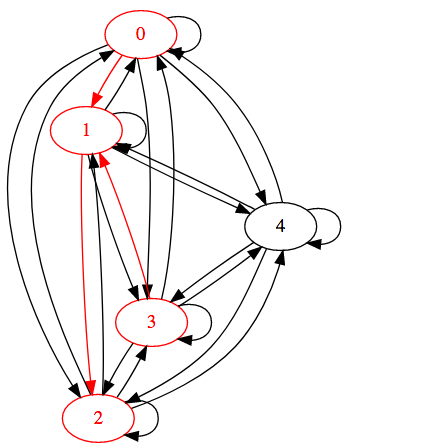
\includegraphics[width=4cm]{graphViz}

%\subsection{Large Neighborhood Search}
%
%Large Neighborhood Search (LNS) is most powerful technique to solve large scale optimization problems. It may not be able to prove optimality but is designed to provide very good solutions in a reasonable runtime. Another interesting motivation for setting up an LNS is that the output solution may not be easy to improve by hand. 
%
%The sample \texttt{TSP\_lns.java} provides an illustration of how to implement a large neighborhood search to solve a tsp. 
%Setting up an LNS requires can be done as follows:
%\begin{lstlisting}
%// object describing which edges to freeze
%SubpathLNS LNS = new SubpathLNS(graph.getNbMaxNodes(),solver);
%// restarts every 30 fails (facultative)
%LNS.fastRestart(new FailCounter(30)); 
%// set up the lns (the last argument indicates whether to restart on every solution) 
%solver.plugMonitor(new LargeNeighborhoodSearch(solver,LNS,false))
%\end{lstlisting} 
%
%The only smart part relies in the implementation of \texttt{INeighbor}. We provide the following implementation
%\begin{lstlisting}
%/**
% * Object describing which edges to freeze and which others to relax in the LNS
% * Relaxes a (sub)path of the previous solution (freezes the rest)
% */
%private class SubpathLNS extends ANeighbor{
%
%	Random rd = new Random(0);
%	int n, nbRL; // number of nodes, counter 
%	UndirectedGraph solution; // object to  store the current best solution
%	int nbFreeEdges = 15; // number of edges which should not be frozen
%
%	protected SubpathLNS(int n, Solver mSolver) {
%		super(mSolver);
%		this.n = n;
%		this.solution = new UndirectedGraph(n,SetType.LINKED_LIST,true);
%	}
%
%	@Override
%	public void recordSolution() {
%		// stores a solution in a graph object
%		for(int i=0;i<n;i++)solution.getNeighOf(i).clear();
%		for(int i=0;i<n;i++){
%			ISet nei = graph.getMandNeighOf(i);
%			for(int j=nei.getFirstElement();j>=0;j=nei.getNextElement()){
%				solution.addEdge(i,j);
%			}
%		}
%	}
%
%	@Override
%	public void fixSomeVariables(ICause cause) throws ContradictionException {
%		// relaxes a sub-path (a set of consecutive edges in a solution)
%		int i1 = rd.nextInt(n);
%		ISet nei = solution.getNeighOf(i1);
%		int i2 = nei.getFirstElement();
%		if(rd.nextBoolean()){
%			i2 = nei.getNextElement();
%		}
%		for(int k=0;k<n-nbFreeEdges;k++){
%			graph.enforceArc(i1,i2,cause);
%			int i3 = solution.getNeighOf(i2).getFirstElement();
%			if(i3==i1){
%				i3 = solution.getNeighOf(i2).getNextElement();
%			}
%			i1 = i2;
%			i2 = i3;
%		}
%	}
%
%	@Override
%	public void restrictLess() {
%		nbRL++;
%		// Eventually increases the size of the relaxes fragment (not necessary)
%		if(nbRL>nbFreeEdges){
%			nbRL = 0;
%			nbFreeEdges += (nbFreeEdges*3)/2;
%		}
%	}
%
%	@Override
%	public boolean isSearchComplete() {
%		return nbFreeEdges>=n;
%	}
%}
%\end{lstlisting}
%
%The main methods to implement are \texttt{recordSolution()} which requires to copy some part of the current solution in internal data structure in order to be able to freeze some edges later. 
%The method \texttt{fixSomeVariables} is called after a restart in order to freeze some variables (here some edges). The method \texttt{restrictLess} does not need to be implemented. It is called some times to suggest considering a larger neighborhood (variable neighborhood search). Finally, \texttt{isSearchComplete} asks whether the search is complete or not. The answer should be \texttt{false} in the general case, unless no variable has been frozen (which may occur in variable large neighborhood search). 


\newpage{}
\section{Appendix : Practical examples}

Examples may be found in the source code in package \texttt{org.chocosolver.samples} 

\subsection{Large scale Hamiltonian cycle : The Knight's Tour Problem}

The Knight's Tour Problem (KTP) is defined over a chessboard and consists of making a chess knight visit every cell exactly once and reach back its original position, where possible moves are given by classical chess rules for the knight. This problem can be seen as a graph problem. Let us introduce an undirected graph for which every vertex is associated with a cell of the chessboard and there is an edge between two vertices if and only if the chess rules allow to travel between the two cells associated with the edge endpoints. The problem then consists of finding a Hamiltonian cycle in this graph. This can be addressed using \texttt{Choco-Graph}. Here is the graph-based CP model of this KTP (with a board length of $200$, which involves a $40,000$-vertex graph) : 
\begin{lstlisting}

import org.chocosolver.graphsolver.GraphModel;
import org.chocosolver.graphsolver.search.strategy.ArcStrategy;
import org.chocosolver.graphsolver.search.strategy.GraphStrategy;
import org.chocosolver.graphsolver.variables.UndirectedGraphVar;
import org.chocosolver.solver.Solver;
import org.chocosolver.util.objects.graphs.UndirectedGraph;
import org.chocosolver.util.objects.setDataStructures.ISet;
import org.chocosolver.util.objects.setDataStructures.SetType;

/**
 * Solves the Knight's Tour Problem
 * <p/>
 * Uses graph variables (light data structure)
 * better with -Xms1048m -Xmx2048m for memory allocation
 * when solving large instances
 *
 *
 * @author Jean-Guillaume Fages
 * @since Oct. 2012
 */
public class KnightTourProblem {

	public static void main(String[] args) {
		boolean[][] matrix;
		boolean closedTour = true; //Open tour (path instead of cycle)
		int boardLength = 100;
		// This generates the boolean incidence matrix of the chessboard graph
		// It is responsible of the high memory consumption of this example
		// and could be replaced by lighter data structure
		if (closedTour) {
			matrix = HCP_Utils.generateKingTourInstance(boardLength);
		} else {
			matrix = HCP_Utils.generateOpenKingTourInstance(boardLength);
		}
		GraphModel model = new GraphModel("solving the knight's tour problem with a graph variable");
		// variables
		int n = matrix.length;
		// graph representing mandatory nodes and edges
		// (linked list data structure as the expected solution is expected to be sparse,
		// every vertex in [0,n-1] is mandatory)
		UndirectedGraph GLB = new UndirectedGraph(model,n,SetType.LINKED_LIST,true);
		// graph representing potential nodes and edges
		// (linked list data structure as its initial value is sparse,
		UndirectedGraph GUB = new UndirectedGraph(model,n,SetType.LINKED_LIST,true);
		for (int i = 0; i < n; i++) {
			for (int j = i + 1; j < n; j++) {
				if (matrix[i][j]) { // adds possible edge
					GUB.addEdge(i, j);
				}
			}
		}
		// creates the graph variable
		IUndirectedGraphVar graph = model.graphVar("G", GLB, GUB);

		// hamiltonian cycle constraint
		model.hamiltonianCycle(graph).post();

		// basically branch on sparse areas of the graph
		Solver solver = model.getSolver();
		solver.setSearch(new GraphStrategy(
			graph, null, new MinNeigh(graph), GraphStrategy.NodeArcPriority.ARCS
		));
		solver.limitTime("20s");

		solver.solve();
		solver.printStatistics();
	}

	//***********************************************************************************
	// HEURISTICS
	//***********************************************************************************

	private static class MinNeigh extends ArcStrategy<UndirectedGraphVar> {
		int n;

		public MinNeigh(UndirectedGraphVar graphVar) {
			super(graphVar);
			n = graphVar.getNbMaxNodes();
		}

		@Override
		public boolean computeNextArc() {
			ISet suc;
			int size = n + 1;
			int sizi;
			from = -1;
			for (int i = 0; i < n; i++) {
				sizi = g.getPotNeighOf(i).size() - g.getMandNeighOf(i).size();
				if (sizi < size && sizi > 0) {
					from = i;
					size = sizi;
				}
			}
			if (from == -1) {
				return false;
			}
			suc = g.getPotNeighOf(from);
			for (int j : suc) {
				if (!g.getMandNeighOf(from).contain(j)) {
					to = j;
					return true;
				}
			}
			throw new UnsupportedOperationException();
		}
	}
}
\end{lstlisting}

The Hamiltonian cycle constraint involves basic filtering but which run incrementally in constant time for each edge removal/enforcing. 
Note that having a undirected model is a key (a directed representation would bring symmetries and increase the search space). 
This model provides the following output (obtained on a usual laptop):
\begin{lstlisting}
** Choco 3.2.1-SNAPSHOT (2014-05) : Constraint Programming Solver, Copyleft (c) 2010-2014
** Solve : solving the knight's tour problem with a graph variable
- Search statistics
	Solutions: 1
	Building time : 2,796s		// time to build the graph variable domain and propagators
	Initialisation : 0,007s
	Initial propagation : 0,039s	// initial propagation runtime
	Resolution : 7,918s			// total solving time
	Nodes: 39 507				// number of branching node is almost the number of nodes in the graph (40,000)
	Backtracks: 1				// good filtering and good search! This model is good on the Hamiltonian cycle problem.
	Fails: 1					
	Restarts: 0
	Max depth: 39 506
	Propagations: 103 963 + 0	// number of incremental propagations + number of non-incremental propagations
	Memory: -20mb			// memory usage of the model (while the input matrix takes >1gb)
	Variables: 3				// graph + default solver constants (ZERO and ONE)
	Constraints: 1				// Hamiltonian cycle constraint (which has 3 incremental propagators)
\end{lstlisting}

If we take a small instance, with a board length of $8$, whence $64$ vertices. 
Here is the print of the graph variable initial domain : 
\begin{lstlisting}

graph_var G
upper bound: // (potential nodes and edges)
nodes : 
[0,63]
neighbors : 
0 -> {17 10 }
1 -> {18 16 11 }
2 -> {19 17 12 8 }
3 -> {20 18 13 9 }
4 -> {21 19 14 10 }
5 -> {22 20 15 11 }
6 -> {23 21 12 }
7 -> {22 13 }
8 -> {25 18 2 }
9 -> {26 24 19 3 }
10 -> {27 25 20 16 4 0 }
11 -> {28 26 21 17 5 1 }
12 -> {29 27 22 18 6 2 }
13 -> {30 28 23 19 7 3 }
14 -> {31 29 20 4 }
15 -> {30 21 5 }
16 -> {33 26 10 1 }
17 -> {34 32 27 11 2 0 }
18 -> {35 33 28 24 12 8 3 1 }
19 -> {36 34 29 25 13 9 4 2 }
20 -> {37 35 30 26 14 10 5 3 }
21 -> {38 36 31 27 15 11 6 4 }
22 -> {39 37 28 12 7 5 }
23 -> {38 29 13 6 }
24 -> {41 34 18 9 }
25 -> {42 40 35 19 10 8 }
26 -> {43 41 36 32 20 16 11 9 }
27 -> {44 42 37 33 21 17 12 10 }
28 -> {45 43 38 34 22 18 13 11 }
29 -> {46 44 39 35 23 19 14 12 }
30 -> {47 45 36 20 15 13 }
31 -> {46 37 21 14 }
32 -> {49 42 26 17 }
33 -> {50 48 43 27 18 16 }
34 -> {51 49 44 40 28 24 19 17 }
35 -> {52 50 45 41 29 25 20 18 }
36 -> {53 51 46 42 30 26 21 19 }
37 -> {54 52 47 43 31 27 22 20 }
38 -> {55 53 44 28 23 21 }
39 -> {54 45 29 22 }
40 -> {57 50 34 25 }
41 -> {58 56 51 35 26 24 }
42 -> {59 57 52 48 36 32 27 25 }
43 -> {60 58 53 49 37 33 28 26 }
44 -> {61 59 54 50 38 34 29 27 }
45 -> {62 60 55 51 39 35 30 28 }
46 -> {63 61 52 36 31 29 }
47 -> {62 53 37 30 }
48 -> {58 42 33 }
49 -> {59 43 34 32 }
50 -> {60 56 44 40 35 33 }
51 -> {61 57 45 41 36 34 }
52 -> {62 58 46 42 37 35 }
53 -> {63 59 47 43 38 36 }
54 -> {60 44 39 37 }
55 -> {61 45 38 }
56 -> {50 41 }
57 -> {51 42 40 }
58 -> {52 48 43 41 }
59 -> {53 49 44 42 }
60 -> {54 50 45 43 }
61 -> {55 51 46 44 }
62 -> {52 47 45 }
63 -> {53 46 }

lower bound:	// (mandatory nodes and edges)
nodes :		
[0,63]		// all vertices are mandatory
neighbors :	// no edge is mandatory
0 -> {}
1 -> {}
2 -> {}
3 -> {}
4 -> {}
5 -> {}
6 -> {}
7 -> {}
8 -> {}
9 -> {}
10 -> {}
11 -> {}
12 -> {}
13 -> {}
14 -> {}
15 -> {}
16 -> {}
17 -> {}
18 -> {}
19 -> {}
20 -> {}
21 -> {}
22 -> {}
23 -> {}
24 -> {}
25 -> {}
26 -> {}
27 -> {}
28 -> {}
29 -> {}
30 -> {}
31 -> {}
32 -> {}
33 -> {}
34 -> {}
35 -> {}
36 -> {}
37 -> {}
38 -> {}
39 -> {}
40 -> {}
41 -> {}
42 -> {}
43 -> {}
44 -> {}
45 -> {}
46 -> {}
47 -> {}
48 -> {}
49 -> {}
50 -> {}
51 -> {}
52 -> {}
53 -> {}
54 -> {}
55 -> {}
56 -> {}
57 -> {}
58 -> {}
59 -> {}
60 -> {}
61 -> {}
62 -> {}
63 -> {}
\end{lstlisting}

After solving the KTP, printing the (value of) the graph variable gives:
\begin{lstlisting}
graph_var G
value: 		// the variable is instantiated
nodes : 
[0,63]		// All vertices belong to the solution graph
neighbors : 
0 -> {17 10 }	// The neighbors of node 0 are nodes 17 and 10
1 -> {18 16 }	//... edges (1,18) and (1,16) belong to the solution graph
2 -> {19 17 }	// ...
3 -> {20 13 }
4 -> {19 14 }
5 -> {22 11 }
6 -> {23 21 }
7 -> {22 13 }
8 -> {25 18 }
9 -> {26 24 }
10 -> {27 0 }
11 -> {28 5 }
12 -> {29 27 }
13 -> {7 3 }
14 -> {31 4 }
15 -> {30 21 }
16 -> {33 1 }
17 -> {2 0 }
18 -> {8 1 }
19 -> {4 2 }
20 -> {35 3 }
21 -> {15 6 }
22 -> {7 5 }
23 -> {38 6 }
24 -> {41 9 }
25 -> {42 8 }
26 -> {36 9 }
27 -> {12 10 }
28 -> {34 11 }
29 -> {44 12 }
30 -> {36 15 }
31 -> {46 14 }
32 -> {49 42 }
33 -> {48 16 }
34 -> {51 28 }
35 -> {45 20 }
36 -> {26 30 }
37 -> {43 47 }
38 -> {55 23 }
39 -> {54 45 }
40 -> {57 50 }
41 -> {56 24 }
42 -> {32 25 }
43 -> {37 60 }
44 -> {61 29 }
45 -> {35 39 }
46 -> {63 31 }
47 -> {62 37 }
48 -> {58 33 }
49 -> {59 32 }
50 -> {56 40 }
51 -> {57 34 }
52 -> {62 58 }
53 -> {63 59 }
54 -> {60 39 }
55 -> {61 38 }
56 -> {50 41 }
57 -> {51 40 }
58 -> {52 48 }
59 -> {53 49 }
60 -> {54 43 }
61 -> {55 44 }
62 -> {52 47 }
63 -> {53 46 }
\end{lstlisting}

\subsection{Solving the Traveling Salesman Problem}

The sample \texttt{TSP\_CP\_Solver} applies $30$ seconds of LNS and $30$ seconds of classical DFS of the CP model for solving the TSP. 
The CP model for the TSP is the following:
\begin{lstlisting}
// variables
totalCost = VariableFactory.bounded("obj", 0, 99999999, solver);
// creates a graph containing n nodes
UndirectedGraph GLB = new UndirectedGraph(solver, n, SetType.LINKED_LIST, true);
UndirectedGraph GUB = new UndirectedGraph(solver, n, SetType.SWAP_ARRAY, true);
// adds potential edges
for (int i = 0; i < n; i++) {
	for (int j = i + 1; j < n; j++) {
		GUB.addEdge(i, j);
	}
}
graph = model.undirected_graph_var("G", GLB, GUB, solver);

// constraints : TSP basic model + lagrangian relaxation (after a first solution has been found)
model.tsp(graph, totalCost, costMatrix, 2));
\end{lstlisting}

Note that in the exact (DFS) model, the Lagrangian relaxation is triggered since root node (mode $=1$). 
The search procedure varies from one model to the other (see the sample files). 
The output on the \texttt{bier127} instance, involving a complete graph of $127$ vertices, is the following:

\begin{lstlisting}
** Choco 3.2.1-SNAPSHOT (2014-05) : Constraint Programming Solver, Copyleft (c) 2010-2014
** Solve : TSP_lns
solution found : obj = 141339
solution found : obj = 138636
solution found : obj = 137046
solution found : obj = 136912
solution found : obj = 136263
...
solution found : obj = 118528
solution found : obj = 118502
solution found : obj = 118442
solution found : obj = 118386
solution found : obj = 118374
solution found : obj = 118326
solution found : obj = 118282
- Search statistics
	Solutions: 165
	Minimize obj = 118282,
	Building time : 0,123s
	Initialisation : 0,007s
	Initial propagation : 0,333s
	Resolution : 30,014s
	Nodes: 2 348
	Backtracks: 2 960
	Fails: 1 498
	Restarts: 137
	Max depth: 126
	Propagations: 19 981 + 0
	Memory: -6mb
	Variables: 4
	Constraints: 1
Best solution found : 118282 (but no optimality proof)
** Choco 3.2.1-SNAPSHOT (2014-05) : Constraint Programming Solver, Copyleft (c) 2010-2014
** Solve : TSP_exact
solution found : obj = 118282
- Search statistics
	Solutions: 1
	Minimize obj = 118282,
	Building time : 0,003s
	Initialisation : 0,000s
	Initial propagation : 0,039s
	Resolution : 1,077s
	Nodes: 129
	Backtracks: 257
	Fails: 128
	Restarts: 0
	Max depth: 23
	Propagations: 1 535 + 0
	Memory: -1mb
	Variables: 4
	Constraints: 1
Optimality proved with exact CP approach
\end{lstlisting}

As you can see, the LNS is a powerful tool to find very good (sometimes optimal) solutions, and we can then use a classical DFS approach to perform the optimality proof. 

\subsection{Finding a Directed Acyclic (sub)Graph}

We now consider the problem of finding a DAG comprised between two input graphs (initial domain) and such that the number of arcs is maximal. 
This problem can be stated through the following program:
\begin{lstlisting}
import org.chocosolver.graphsolver.GraphModel;
import org.chocosolver.graphsolver.variables.DirectedGraphVar;
import org.chocosolver.solver.Model;
import org.chocosolver.solver.variables.IntVar;
import org.chocosolver.util.objects.graphs.DirectedGraph;
import org.chocosolver.util.objects.setDataStructures.SetType;

public class DAGProblem {

	public static void main(String[] args){
		// input graph
		int n = 5;
		// VARIABLE COUNTING THE NUMBER OF ARCS
		GraphModel model = new GraphModel();
		IntVar nbArcs = model.intVar("arcCount", 0, n * n, true);
		// GRAPH VARIABLE : initial domain (every node belongs to the solution)
		DirectedGraph GLB = new DirectedGraph(model, n, SetType.BITSET, true);
		DirectedGraph GUB = new DirectedGraph(model, n, SetType.BITSET, true);
		GLB.addArc(0,1); // some arbitrary mandatory arcs
		GLB.addArc(1,2);
		GLB.addArc(3,1);
		for (int i = 0; i < n; i++) {
			for (int j = 0; j < n; j++) {
				GUB.addArc(i, j);		// potential edge
			}
		}

		DirectedGraphVar dag = model.digraphVar("dag", GLB, GUB);

		// CONSTRAINTS
		model.noCircuit(dag).post();
		model.nbArcs(dag, nbArcs).post();

		model.setObjective(Model.MAXIMIZE,nbArcs);
		while (model.getSolver().solve()){
			System.out.println("new solution found : "+nbArcs);
			System.out.println(dag);
		}
	}
}
\end{lstlisting}

This provides the following output:

\begin{lstlisting}
graph_var dag
value: 
nodes : 
[0,4]
successors : 
0 -> {1 2 3 4 }
1 -> {2 4 }
2 -> {4 }
3 -> {1 2 4 }
4 -> {}

** Choco 4.0.0 (2016-06) : Constraint Programming Solver, Copyleft (c) 2010-2016
- Model[Graph Model] features:
	Variables : 2
	Constraints : 2
	Default search strategy : yes
	Completed search strategy : no
- Complete search - 1 solution found.
	Model[Graph Model]
	Solutions: 1
	Maximize arcCount = 10,
	Building time : 0,000s
	Resolution time : 0,066s
	Nodes: 23 (349,7 n/s) 
	Backtracks: 45
	Fails: 22
	Restarts: 0

Process finished with exit code 0
\end{lstlisting}


\bibliographystyle{elsarticle-num}
\bibliography{ChocoGraph}

\end{document}